\section{Cloud Liefermodelle}
\begin{figure}[H]
  \centering
    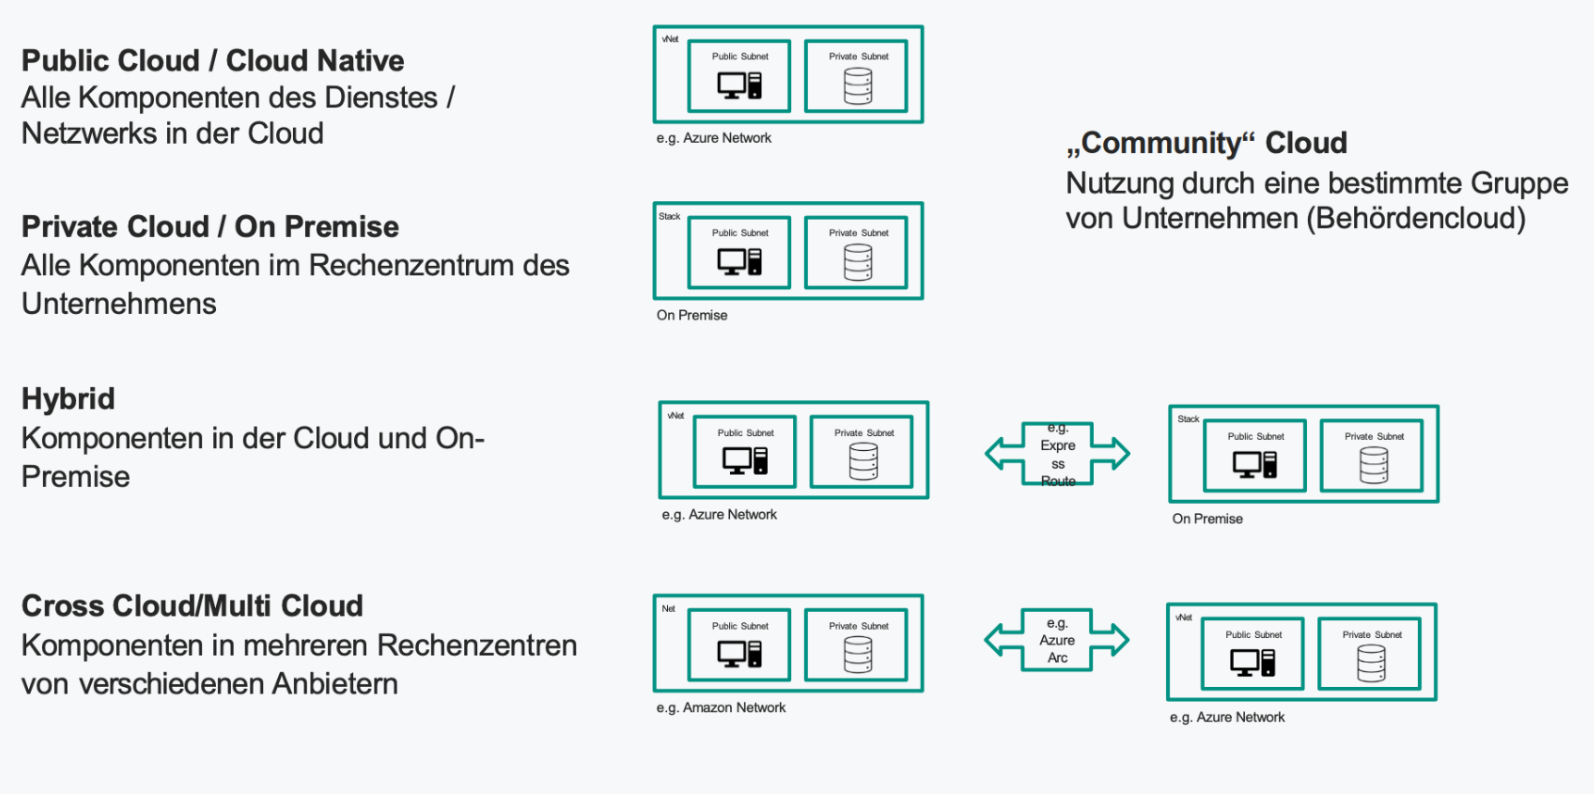
\includegraphics[width=\textwidth]{assets/images/coludliefermodell}
\end{figure}
\begin{table}[H]
    \centering
    \renewcommand{\arraystretch}{1.6}
    \begin{tabular}{|p{2.5cm}|p{2.8cm}|p{3.8cm}|p{3cm}|p{3.2cm}|}
        \hline
        \textbf{Modell}
            & \textbf{Kosten}
            & \textbf{Sicherheit}
            & \textbf{Customization / Flexibilität}
            & \textbf{Notwendige Ressourcen} \\
        \hline
        \textbf{Public Cloud}
            & Kostengünstigste Architektur
            & Hoher Sicherheitsstandard, keine volle Kontrolle (reicht möglicherweise nicht aus)
            & Begrenzt, abhängig vom Dienst des Cloud-Service-Providers (CSP)
            & Kein detailliertes Infrastruktur-Know-how erforderlich \\
        \hline
        \textbf{Private Cloud}
            & Teuerste Architektur
            & Volle Eigenverantwortung: nichts ist vorkonfiguriert, alle Sicherheitsstandards müssen selbst auf eigene Kosten umgesetzt werden
            & Infrastruktur kann beliebig konfiguriert werden
            & Detailliertes Know-how für alle erforderlichen Infrastrukturebenen erforderlich \\
        \hline
        \textbf{Hybride Cloud}
            & Könnte je nach Bedarf Vorteile haben
            & Alle Sicherheitsstandards umsetzbar. Die Verbindung zur Cloud muss gesichert sein
            & Alle Möglichkeiten beider Architekturen
            & Detailliertes Know-how für alle erforderlichen Infrastrukturebenen erforderlich \\
        \hline
    \end{tabular}
    \caption{Vergleich der Cloud-Bereitstellungsmodelle}
    \label{tab:cloud-modelle}
\end{table}